\chapter{Agile Software Engineering}
For the past 50 years, software engineering was primarily focused on plan-driven development, which included:

\begin{itemize}
    \item Detailed project planning (a particularly heavy part)
    \item Requirement specification (also a very intensive part)
    \item Analysis and design methods
    \item Comprehensive system documentation
    \item Formal quality assurance
\end{itemize}

\noindent At the beginning of the new millennium, a manifesto for agile software development was published, emphasizing:

\begin{itemize}
    \item \textbf{Individuals and interactions} over processes and tools
    \item \textbf{Working software} over comprehensive documentation (even though documentation is useful for those who will modify the code later, making it detailed is very costly)
    \item \textbf{Customer collaboration} over contract negotiation (to include the customer in the software development process)
    \item \textbf{Responding to change} over following a plan (since no one can predict the future)
\end{itemize}

The radically new perspective of Agile is to move away from thinking about applications the way they were previously thought of and instead try to align with how users think about the system (as a set of functionalities). One of the Agile principles is \textbf{Incremental Development}: it involves selecting a few functionalities and then implementing them.

\begin{figure} [H]
    \centering
    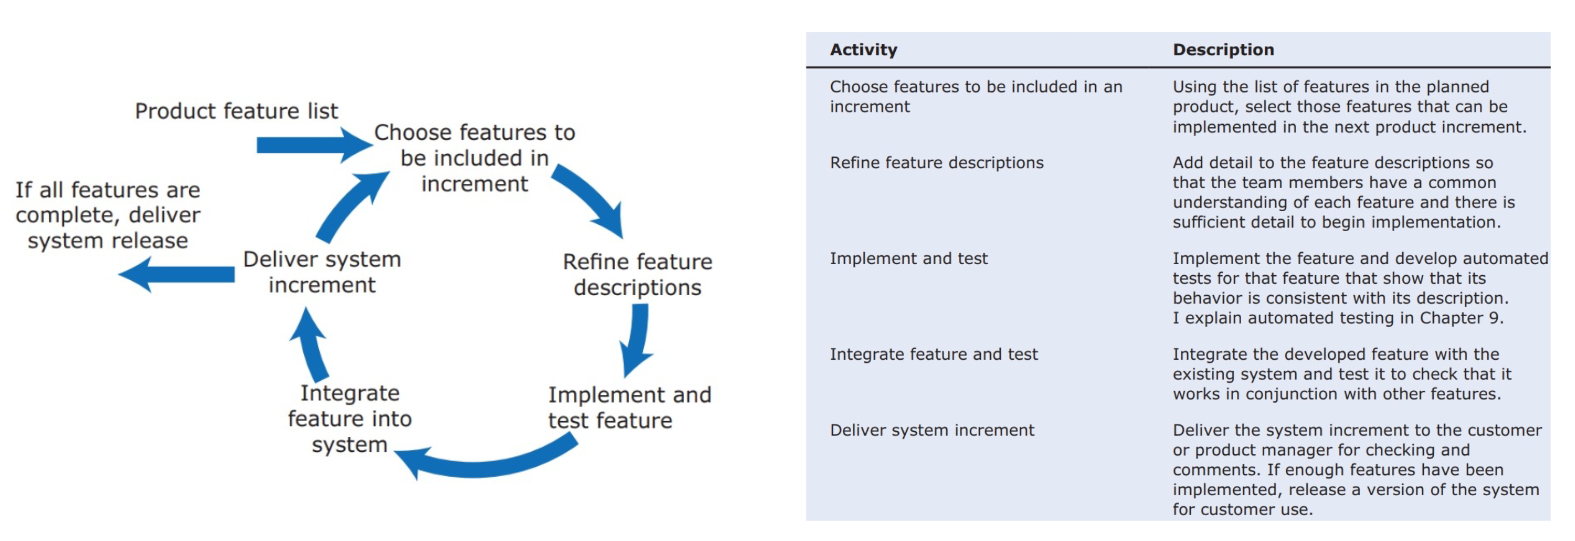
\includegraphics[width=1\textwidth]{images/Agile/CICD.png}
    \caption{Continuous Integration and Continuous Deployment cycle}
    \label{fig:CICD}
\end{figure}

This cycle is then repeated until the final system is completed. These rounds, where we implement features, can sometimes fail, either due to a misinterpretation of required functionalities or because the customer changes their mind. This process, which can be visualized as a pipeline, is called \textbf{Continuous Integration and Continuous Delivery/Continuous Deployment} (CICD). \\

\noindent Here are twelve more \textbf{Agile principles}:

\begin{itemize}
    \item Our highest priority is to satisfy the customer through \textit{early and continuous delivery of valuable software}. (as soon as there's a usable piece of software, it should be deployed)
    \item \textbf{Welcome changing requirements}, even late in development. Agile processes harness change for the customer's competitive advantage. (it is unrealistic to have a full and complete set of functionalities from users at the beginning of development. Programmers should adopt a mindset that embraces changing requirements)
    \item \textbf{Deliver working software frequently}, from a couple of weeks to a couple of months, with a preference for the shorter timescale. (CICD pipeline)
    \item Business people and developers must \textbf{work together} daily throughout the project.
    \item The most efficient and effective method of conveying information to and within a development team is face-to-face conversation.
    \item \textbf{Working software is the primary measure of progress}. (not the delivery of new documentation or specifications)
    \item Agile processes promote sustainable development. The sponsors, developers, and users should be able to maintain a constant pace indefinitely.
    \item Continuous attention to technical excellence and good design enhances agility.
    \item \textbf{Simplicity}—the art of maximizing the amount of work not done—is essential.
    \item The best architectures, requirements, and designs emerge from \textbf{self-organizing teams}. (rather than having separate teams in different rooms)
    \item At regular intervals, the \textbf{team reflects} on how to become more effective, then tunes and adjusts its behavior accordingly. (periodically evaluate and adjust practices)
\end{itemize}


\section{Extreme Programming}

Extreme Programming (XP) is one of the techniques proposed as part of Agile methodology. The key points of XP are shown in the following image:

\begin{figure} [H]
    \centering
    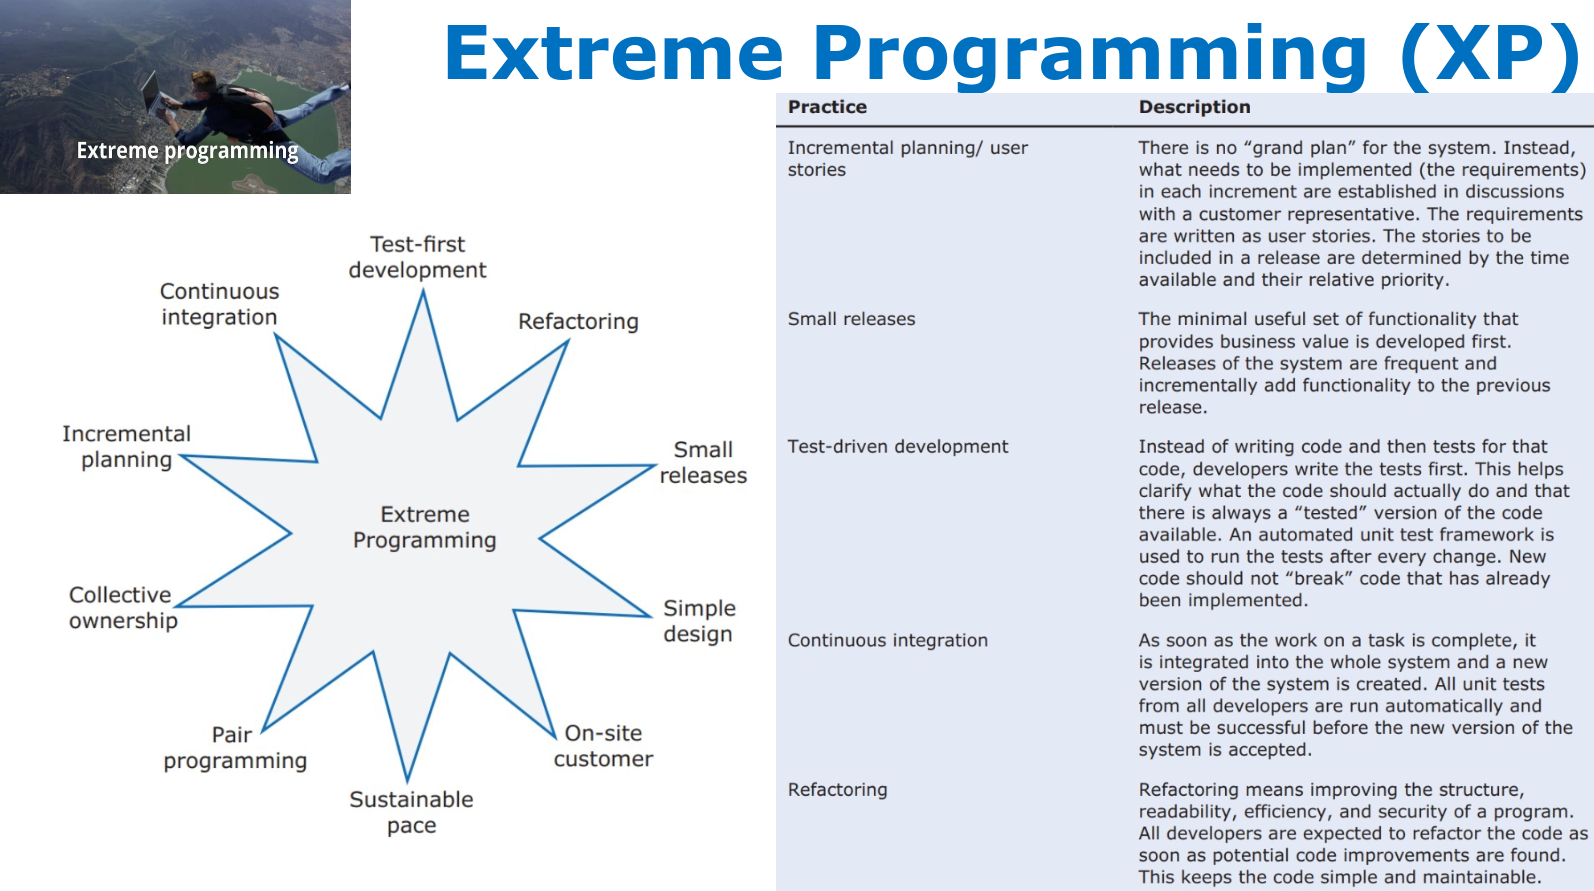
\includegraphics[width=1\textwidth]{images/Agile/ExtremeProgramming.png}
    \caption{Extreme Programming principles}
    \label{fig:extremeprogramming}
\end{figure} 

\section{Scrum}

Scrum is a \textbf{lightweight framework} that helps individuals, teams, and organizations generate value through adaptive solutions to complex problems. The Scrum framework contains a set of principles and rules to follow in order to achieve a common goal.

The motivation behind Scrum is that software company managers need information that helps them understand the cost of developing a software product, the development timeline, and when the product can be brought to market. Plan-driven development provides this information through long-term development plans that identify deliverables—items the team will deliver and when these will be delivered. However, plans always change, making long-term plans unreliable, except for short-term planning.

Scrum is based on \textbf{Empiricism}, which asserts that knowledge comes from experience and that decisions should be made based on observation. It is also rooted in \textbf{Lean thinking}, which focuses on reducing waste and emphasizing essentials. Scrum employs an iterative, incremental approach to optimize predictability and control risk. The pillars of Scrum are:

\begin{itemize}
    \item \textbf{Transparency}: The progress and work should be visible to those performing the work and those receiving the work.
    \item \textbf{Inspection}: Scrum artifacts and progress toward agreed goals must be frequently and diligently inspected to detect potentially undesirable variances or problems.
    \item \textbf{Adaptation}: If any aspects of a process deviate (e.g., new requirements) beyond acceptable limits, or if the resulting product is unacceptable, the process being applied or the materials being produced must be adjusted. These adjustments should be made as soon as possible to minimize further deviation.
\end{itemize}

Successful use of Scrum depends on people becoming more proficient in living its five core values: \textbf{Commitment} (respect deadlines), \textbf{Focus}, \textbf{Openness} (being open to new solutions), \textbf{Respect} (for teammates and others), and \textbf{Courage} (to propose new solutions that better align the product with its vision).

\subsection{Scrum Team}

A \textbf{self-organizing team} coordinates its work by discussing tasks and reaching a consensus on who should do what. This minimizes the involvement of engineers in external interactions with management and customers. The team makes its own decisions on schedules and deliverables.

\textbf{External interactions} refer to interactions team members have with individuals outside the team. In Scrum, the idea is that developers should focus on development, while only the Scrum Master and Product Owner should handle external interactions. The goal is for the team to focus on software development without external interference or distractions.

\subsubsection{Product Owner}

The Product Owner is responsible for ensuring that the development team stays focused on building the product rather than getting sidetracked by technically interesting but less relevant work. In product development, the Product Manager typically assumes the Product Owner role. \\

Product-focused external interactions are managed by the Product Owner.

\subsubsection{Scrum Master}

The Scrum Master is an expert in Scrum whose job is to guide the team in effectively using the Scrum method. Scrum developers emphasize that the Scrum Master is not a traditional project manager but rather a coach for the team. They have authority within the team regarding how Scrum is used. In many companies, the Scrum Master also takes on some project management responsibilities. \\

In all but the smallest product development companies, development teams must report progress to company management. A self-organizing team needs to appoint someone to handle these responsibilities. Because maintaining continuity in communication with people outside the group is crucial, rotating these activities among team members is not a viable approach. Although the Scrum developers did not envision the Scrum Master also assuming project management responsibilities, in many companies, \textit{the Scrum Master takes on project management tasks} because they have the best understanding of the work in progress and are in the best position to provide accurate information and project plans. \\

Team-focused external interactions are managed by the Scrum Master.

\subsubsection{Developers}

Self-organizing teams make their own decisions, working by discussing issues and reaching a consensus. The ideal \textbf{Scrum team size} is between 5 and 8 people. Teams need to tackle diverse tasks, often requiring members with different skills, such as networking, user experience, database design, and more. They also typically include individuals with varying levels of experience. A team of 5 to 8 people is large enough to be diverse yet small enough to communicate informally and effectively, allowing for agreement on team priorities.

The advantage of a self-organizing team is that it can become cohesive and adapt to change. Because the team, rather than individuals, takes responsibility for the work, it can manage transitions when team members leave or join. Effective communication within the team means that members inevitably learn about each other’s areas of expertise. \\

The developers of Scrum assumed that teams would be co-located, working in the same space to communicate informally. Daily scrums help team members stay updated on what’s been done and what others are working on. However, two assumptions behind the daily scrum are not always correct: 
\begin{itemize}
    \item Scrum assumes that the team is made up of full-time workers sharing a workspace. In reality, team members may work part-time or in different locations. For student project teams, members may take different classes at different times.
    \item Scrum assumes that all team members can attend a morning meeting to coordinate the day’s work. However, some members may work flexible hours (e.g., due to childcare responsibilities) or may work on several projects simultaneously.
\end{itemize}

\subsection{Artifacts}

\subsubsection{Product Backlog}

The product backlog is a list of tasks that need to be completed to develop the product. This to-do list of items is reviewed and updated before each sprint.

\begin{figure} [H]
    \centering
    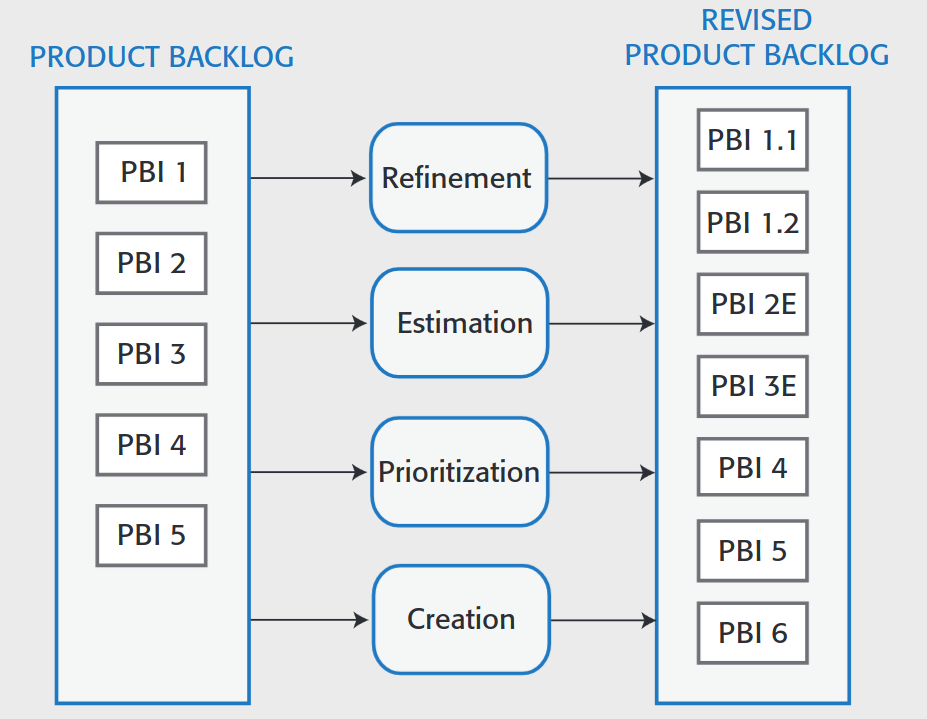
\includegraphics[width=0.8\textwidth]{images/Agile/ProductBacklog.png}
    \caption{Product backlog during the action process}
    \label{fig:productbacklog}
\end{figure} 

As illustrated in the image above, items that are to be implemented are first selected and prioritized. According to their priorities, they are sorted and will be implemented in the next sprint. Below are some examples of product backlog items:

\begin{itemize}
    \item \textit{As a teacher, I want to be able to configure the group of tools that are available to individual classes.} (feature)
    \item \textit{As a parent, I want to be able to view my children's work and the assessments made by their teachers.} (feature)
    \item \textit{As a teacher of young children, I want a pictorial interface for children with limited reading ability.} (user request)
    \item \textit{Implement encryption for all personal user data.} (engineering improvement)
\end{itemize}

\newpage

\noindent Product backlog items can exist in different states:

\begin{itemize}
	\item \textbf{Ready for consideration}: High-level ideas and feature descriptions are under consideration for inclusion in the product. These are tentative and may change or not be included in the final product.
	\item \textbf{Ready for refinement}: The team agrees that this is an important item to be implemented in the current development cycle. There is a reasonably clear definition of what is required, though further refinement is needed.
	\item \textbf{Ready for implementation}: The product backlog item has enough detail for the team to estimate the effort required and begin implementation. Dependencies on other items are also identified.
\end{itemize}

\subsubsection{Sprint Backlog}

The sprint backlog is a focused list of tasks selected from the product backlog that the team commits to completing during the sprint. It is created during sprint planning, where items are chosen based on the sprint goal and broken down into smaller, actionable tasks.

Unlike the product backlog, which contains all potential features and improvements, the sprint backlog is \textbf{limited to what can be achieved within the sprint’s time frame}. As the sprint progresses, the team updates the sprint backlog to track completed tasks and any changes that arise.

The sprint backlog helps the team stay aligned with their sprint goal and manage progress efficiently. Tools like burn-down charts are often used to visualize the remaining work and time in the sprint.

\subsection{Scrum Events}

In Scrum, software is developed in fixed-length periods called \textbf{sprints}, typically lasting 2-4 weeks. During a sprint, the team holds daily meetings (Scrums) to review progress and update the list of incomplete work items. A sprint aims to produce a ‘\textit{shippable product increment},’ meaning that the developed software should be complete and ready to deploy. Sprints are \textbf{timeboxed}, meaning development stops at the end of the sprint, regardless of whether all work has been completed. The team works on items from the product backlog during a sprint. \\

There are three main types of \textbf{sprint activities}:
\begin{itemize}
    \item \textbf{Sprint Planning}: The team selects the work items to be completed during the sprint, and if necessary, refines them to create a sprint backlog. This planning session should not last longer than a day at the start of the sprint.
    \item \textbf{Sprint Execution}: The team works to implement the sprint backlog items. If it becomes impossible to complete all items, the sprint is not extended; instead, unfinished items are returned to the product backlog for future sprints.
    \item \textbf{Sprint Review}: The team and possibly external stakeholders review the completed work. They reflect on what went well, what went wrong, and how to improve their work processes.
\end{itemize}

\begin{figure} [H]
    \centering
    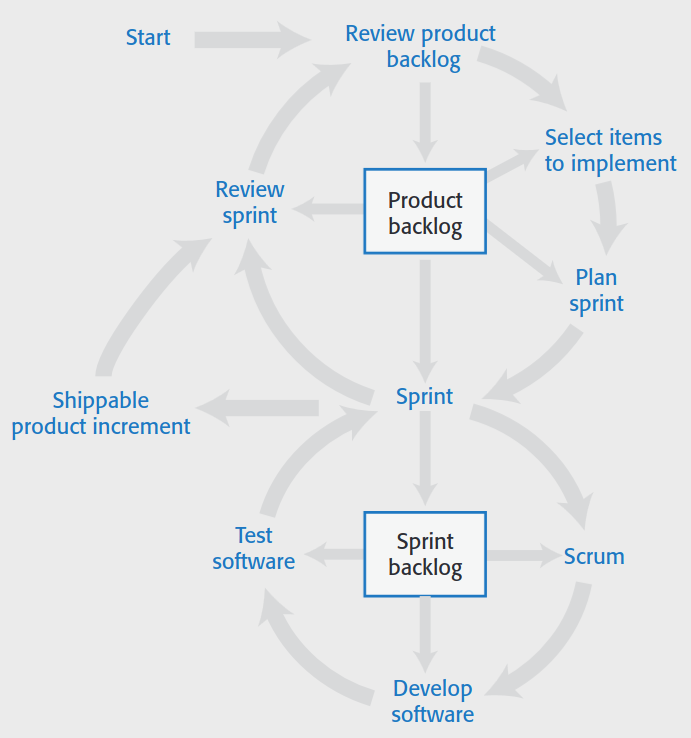
\includegraphics[width=0.7\textwidth]{images/Agile/ScrumCycle.png}
    \caption{Sprint activities within the Scrum cycle}
    \label{fig:scrumcycle}
\end{figure} 

\subsubsection{Sprint Planning}

Sprint planning involves establishing an agreed sprint goal, which may focus on software functionality, support, performance, or reliability. To define the goal, the team selects which items from the product backlog should be implemented. The outcome of this process is a \textbf{sprint backlog}, a more detailed version of the product backlog, listing the tasks to be completed during the sprint. \\

Throughout the sprint, the team holds \textbf{daily Scrum meetings} to coordinate their work. These meetings, often called \emph{scrums}, are short and typically held at the beginning of the day. During the meeting, each team member shares their progress, any problems encountered, and their plans for the day. This ensures that everyone on the team knows what is happening and allows for quick re-planning if needed. Scrum meetings should remain short and focused. To avoid prolonged discussions, they are sometimes held as ‘stand-up’ meetings, where no chairs are provided. \\

During a Scrum, the sprint backlog is reviewed, completed items are removed, and new items may be added as new information arises. The team then decides which team member will work on specific sprint backlog items for the day.

\subsubsection{Sprint Execution}

Scrum does not prescribe specific technical agile activities to be used during a sprint, but two practices are commonly recommended by agile software engineers:

\begin{itemize}
    \item \textbf{Test Automation}: As much testing as possible should be automated. A suite of executable tests should be developed, which can be run at any time to ensure software quality.
    \item \textbf{Continuous Integration}: Whenever changes are made to software components, they should be immediately integrated with the other components to form a complete system. This system should then be tested to check for any unanticipated issues from component interactions.
\end{itemize}

\subsubsection{Sprint Review}

At the end of each sprint, the team conducts a sprint review meeting, involving all team members. The meeting reviews whether the sprint goal was met, addresses any new issues that arose during the sprint, and provides a chance for the team to reflect on how to improve their work process. \\

The product owner has the authority to decide whether the sprint goal has been achieved. They confirm whether the implementation of the selected product backlog items is complete. Additionally, the sprint review should include a process review where the team reflects on how they’ve used Scrum and discusses how to improve productivity in the next sprint.

\subsection{Execution}

Depending on the state of the item, there are different possible actions:

\begin{itemize}
	\item \textbf{Refinement}: Existing PBIs are analyzed and refined to create more detailed PBIs. This may lead to the creation of new product backlog items.
	\item \textbf{Estimation}: The team estimates the amount of work required to implement a PBI and adds this assessment to each analyzed PBI.
	\item \textbf{Creation}: New items are added to the backlog. These may include new features suggested by the product manager, required feature changes, engineering improvements, or process activities such as assessing development tools that might be used.
    \item \textbf{Prioritization}: New items are prioritized within the backlog. These may also include new features suggested by the product manager, required feature changes, engineering improvements, or process activities such as assessing development tools that might be used.
\end{itemize}

We can see the effects of these actions in Figure \ref{fig:productbacklog}. There are metrics that we can apply to PBIs in order to choose the next state or action. The following factors are usually considered:

\begin{itemize}
\item \textbf{Effort required}: This may be expressed in person-hours or person-days, i.e., the number of hours or days it would take one person to implement that PBI. This is not the same as calendar time, as several people may work on an item, which can shorten the calendar time required.
\item \textbf{Story points}: Story points are an arbitrary estimate of the effort involved in implementing a PBI, taking into account the size of the task, its complexity, the technology that may be required, and the ‘unknown’ characteristics of the work. They were originally derived by comparing user stories but can be used for estimating any kind of PBI. Story points are estimated relatively; the team agrees on the story points for a baseline task, and other tasks are estimated by comparison with this, e.g., more/less complex, larger/smaller, etc.
\end{itemize}
